\documentclass[preprint,12pt]{elsarticle}

\usepackage{hyperref}
\usepackage{graphicx}
\usepackage{subcaption}
\usepackage{amssymb}
\usepackage{amsmath}
\usepackage{multirow}
\usepackage{relsize}
\usepackage[utf8]{inputenc}
\usepackage{cleveref}
\usepackage{algorithm}
\usepackage[noend]{algpseudocode}
\usepackage[section]{placeins}
\usepackage{booktabs}
\usepackage{physics}
\usepackage{breqn}

% For the TODOs
\usepackage{xcolor}
\usepackage{xargs}
\usepackage[colorinlistoftodos,textsize=footnotesize]{todonotes}
\newcommand{\todoin}{\todo[inline]}
% from here: https://tex.stackexchange.com/questions/9796/how-to-add-todo-notes
\newcommandx{\unsure}[2][1=]{\todo[linecolor=red,backgroundcolor=red!25,bordercolor=red,#1]{#2}}
\newcommandx{\change}[2][1=]{\todo[linecolor=blue,backgroundcolor=blue!25,bordercolor=blue,#1]{#2}}
\newcommandx{\info}[2][1=]{\todo[linecolor=OliveGreen,backgroundcolor=OliveGreen!25,bordercolor=OliveGreen,#1]{#2}}

%Boldtype for greek symbols
\newcommand{\teng}[1]{\ensuremath{\boldsymbol{#1}}}
\newcommand{\ten}[1]{\ensuremath{\mathbf{#1}}}

\usepackage{lineno}

\journal{}

\begin{document}

\begin{frontmatter}

  \title{Rigid fluid coupling}
  \author[IITB]{Adepu Dinesh \corref{cor1}}
  \ead{adepu.dinesh.a@gmail.com} \author[IITB]{Prabhu Ramachandran}
  \ead{prabhu@aero.iitb.ac.in} \address[IITB]{Department of Aerospace
    Engineering, Indian Institute of Technology Bombay, Powai, Mumbai 400076}

\cortext[cor1]{Corresponding author}

\begin{abstract}
  In this paper, a new particle-based fluid–rigid-body interaction schemes are
  utilised to model violent free-surface flow problems. A variant of Discrete
  element method (DEM), surface aware DEM (SADEM) is proposed to handle the
  contact between irregular bodies, while the fluid phase is modeled using
  corrected transport velocity formulation (CTVF) of smoothed particle
  hydrodynamics (SPH). The accuracy the SADEM-CTVF framework are evaluated via
  several numerical examples involving both analytical and experimental.
  Surface aware DEM is validated using using numerical examples including: (1)
  A free and controlled sliding of a cube, (2) A 2d rolling disc. Further, an
  experimental benchmark, collapse of a stack of cylinders in a dam under
  gravity is considered, three rigid bodies hitting. While the coupling method
  is validated by modeling (1) water-entry of a sphere, (2) 3d dam breaking
  flow hitting stacked cubes. The results indicate that the current method can
  effectively model irregular bodies in a fluid flow.
\end{abstract}

\begin{keyword}
%% keywords here, in the form: keyword \sep keyword
{XXX}, {XXX}, {XXX}

%% MSC codes here, in the form: \MSC code \sep code
%% or \MSC[2008] code \sep code (2000 is the default)

\end{keyword}

\end{frontmatter}

% \linenumbers

\section{Introduction}
\label{sec:intro}

Arbitrary shaped rigid bodies in fluid flows in nature. Debris flowing,
particle transport chemical industries, food processing, in natural hazard
where the bodies are capable of doing catastrophic damage while being
sedimented. In ice-sea modeling. Study of such physics is hard to model, as
the two-way coupling is nonlinear. Many different models were proposed to
handle the current physics.


In meshless methods, MPS-DEM \cite{guo2017numerical} and SPH-DEM
\cite{canelas2016sph} are two ways of modeling the physics. Where Moving
Particle Semi-implicit (MPS) method and smoothed particle hydrodynamics (SPH)
are utilized to study the fluid dynamics, while the Discrete Element Method
(DEM) is used to model the interaction among the rigid bodies and finally both
SPH and MPS are coupled with the rigid bodies to handle the two way coupling.
In addition to DEM alone to model the rigid-rigid interaction, there are also
works where SPH \cite{amicarelli2015smoothed} itself is used to model the
interaction. But it lacks to incorporate the friction between the bodies. In
the current work we have used SPH to model the fluid dynamics.


The SPH method is a meshless numerical method originally proposed by
\citet{monaghan-gingold-stars-mnras-77} and \citet{lucy1977numerical} to model
astrophysics problems. It is fairly success in modeling physics ranging
different fields, \citet{monaghan-review:2005} provides a detailed review of
SPH and its applications. structural dynamics, FSI, fracture to note a few.
SPH has been extensively applied to model the dynamics of fluid in two way
rigid fluid coupling. There are several SPH variants in which the fluid flow
can be modeled. \citet{canelas2016sph} uses WCSPH in rigid fluid coupling in
modeling two way rigid fluid coupling, ISPH is used in \cite{asai2021fluid},
delta sph in \cite{lyu20223d}. Multiphase flow, where air is considered, to
capture the cavity while the rigid body enters the water section is modeled in
\cite{lyu2021study}. A TVF scheme is currently proposed where the particle
shifting is introduced for better particle distribution leading to less errors
is not yet utilized in modeling the rigid fluid coupling.


All the works above are using DEM to model the rigid-rigid interaction doesn't
consider the shape of the body and fails to model bodies with arbitrary shape.
One of the reasons is the contact force model is between two particles, and
those particles are assumed as spheres and the contact handling is taken care.
This doesn't consider the shape of the surface of the rigid body in place.
Irregular bodies are modeled using many different variations now, one of the
methods is by overlapped sphere method \cite{das2007modeling}, SMR-DEM by
\citet{zhan2021surface}, dilated polyhedral DEM \citet{liu2020new}, Fourier
series-based discrete element method \citet{lai2020fourier}, non-smooth wall
modeling by \citet{amaro2019improvement}, GJK-DEM \cite{wachs2012grains3d},
discrete function representation based DEM \cite{lu2012critical}, level set
DEM method \cite{duriez2021precision}. However, these are complicated to
implement and not particle friendly and the rigid bodies have to discretized
differently to handle the non-smooth boundaries. In the current work we have
extended the contact force model proposed by \citet{mohseni2021particle} to
handle three dimensional problems, we also incorporate the damping model.


In the current work, we propose a new method to handle the collision between
arbitrary shaped rigid bodies. Unlike the approach of Mohseni, the proposed
contact force model is less sensitive to the primary secondary body selection.
And the proposed method is robust and very simple to implement when compared
with the existing techniques (cite zhang, Amaro) in the literature. The
current model tries to eliminate the confusion in choosing the primary and
secondary body in a collision instance. The rigid fluid coupling between CTVF
is new. We explored different rigid fluid coupling strategies by simulating
high density ratio simulations. Several examples are simulated to validate the
current scheme, ranging from simulations compared with FEM, analytical results
as well as experimental. Finally, in the interest of reproducibility and
easier ability for researchers to build on this work, our code is open source
and can be found at \url{https://gitlab.com/pypr/rfc}. We used automan package
\cite{automan2018} to automate all the results generated in the current
manuscript.


Numerical examples, collision of three cubes is initially used to test the
conservation property of the current contact mode while dealing with
non-smooth boundaries. Further, a free and forced sliding of a 3d cube on a
frictional inclined plane, and a rolling cylinder whose analytical solutions
exists are utilised to validate the rigid-rigid contact model frictional
model. A granular collapse of a stack of cylinders is modeled and compared
against the experimental results. In order to validate the two-way rigid fluid
coupled scheme a rigid circular body falling in a steady tank is simulated.
Complex interactions of fluid in a 3D dam breaking with multiple rigid bodies,
is studied and compared with the experimental results of SPH-DCDEM.

\textbf{Random points to be included later}.
\begin{itemize}
\item In the context of modeling the rigid fluid coupling by assuming both of
  them as particles and, these are the few papers. The more relevant concern
  the generalization of the fundamental technique of Koshizuka et al. [6] and
  the inclusion of a state-of-the-art Distributed Contact DEM (DCDEM)
  formulation, similar in concept to those employed by both Zhang et al. [14]
  and Ren et al. [15]. A delta -SPH [16] term is added to the continuity equation,
  controlling the density field fluctuations and contributing for the
  mitigation of known solid–fluid interface deficiencies [17], particularly
  the development of a hydrophobic area that results in a reorganization of
  the fluid particle positions.The current work
\item A one way coupling is done by xxxx. Then an semi empirical model is used
  to find the force on the discrete elements by stokes law or other laws. Then
  a two way coupling is introduced by Zhang, also Monaghan did the same
  approach.
\end{itemize}



\FloatBarrier%
\section{Fluid dynamics}
\label{sec:fluid-dynamics}

\todoin{Connor FSI}

\subsection{Governing equations}
\label{sec:governing-eqns-fluid-dynamics}

SPH discretization of the modified governing equations are given by:
\begin{equation}
  \label{eq:sph-discretization-continuity}
  \frac{\tilde{d}\rho_a}{dt} = \sum_{b} \; \frac{m_b}{\rho_{b}} \; (
  \rho_{a} \; \tilde{\ten{u}}_{ab} \; + \;
  (\rho \; (\tilde{\ten{u}} \; - \;
  \ten{u}))_{ab}) \; \cdot \nabla_{a} W_{ab},
\end{equation}
\begin{multline}
  \label{eq:sph-momentum-fluid}
  \frac{\tilde{d}\ten{u}_{a}}{dt} = - \sum_{b} m_b \bigg[
  \bigg(\frac{p_a}{\rho_a^2} + \frac{p_b}{\rho_b^2}\bigg) \ten{I}
   \bigg]
  \cdot \nabla_{a} W_{ab} + \\
  \sum_{b} m_b \frac{4 \eta \nabla W_{ab}\cdot
    \ten{r}_{ab}}{(\rho_a + \rho_b) (r_{ab}^2 + 0.01 h_{ab}^2)} \ten{u}_{ab} +
  \ten{g}_{a},
\end{multline}


\newpage
~\newpage
~\newpage


\FloatBarrier%
\section{Rigid body dynamics}
\label{sec:rbd}

\newpage
~\newpage
The rigid body is discretized into particles with equal spacing each particle
with mass $m_i$ and density $\rho_i$. Rigid body has a total 6 degrees of
freedom (DOF), divided into $3$ translational and $3$ rotational.

The state of the rigid body at a given time (t) can described using position
and velocity of the center of mass ($\ten{x}_{cm}$), velocity of center of
mass ($\ten{v}_{cm}$), a rotation matrix ($\ten{R}$), to define the three
rotational degrees of freedom and angular velocity($\teng{\omega}$). The
center of mass is computed with
\begin{equation}
  \label{eq:center_of_mass}
  \ten{x}_{cm} = \frac{\sum_i m_i \; \ten{x}_{i} }{\sum_i m_i }
\end{equation}

The equations governing the dynamics of rigid body are, balance of linear and
angular momentum given by,
\begin{equation}
  \label{eq:balance_linear_mom}
  \frac{d \; (M \ten{v}_{cm})}{d t} = \sum_i \ten{F}_i,
\end{equation}
\begin{equation}
  \label{eq:balance_angular_mom}
  \frac{d \ten{L}}{d t} = \teng{\tau}_{cm}
\end{equation}
where $\teng{\tau}_{cm}$ is the torque about center of mass due to forces on the
particles,
\begin{equation}
  \label{eq:torque}
  \teng{\tau}_{cm} = \sum_i \ten{F}_i \times (\ten{r}_{cm} - \ten{r}_{i})
\end{equation}
and $\ten{L}$ is the angular momentum of the rigid body about center of mass,
computed as
\begin{equation}
  \label{eq:moi}
  \teng{L} =
  \sum_i \; \ten{r}_i \times \; (\ten{\omega} \times \ten{r}_i)
  = \sum_i \; m_i \; [(\ten{r} \cdot \ten{r}) \ten{I} - \ten{r} \otimes \ten{r}]
\end{equation}
\begin{equation}
  \label{eq:omega_compute}
  \teng{\omega} = \textit{\teng{I}}^{-1} \; \ten{L}
\end{equation}


The state of the rigid body at next time step is evolved through the
integration of governing \cref{eq:balance_linear_mom,eq:balance_angular_mom},
finding the linear velocity of the center of mass $\ten{v}_{cm}$ and angular
momentum $\ten{L}$ at the next timestep as,
\begin{equation}
  \label{eq:lin_pos_cm_update}
  \ten{x}_{cm}^{n+1} = \ten{x}_{cm}^{n} + \ten{v}_{cm}^{n} \; \Delta t
\end{equation}
\begin{equation}
  \label{eq:lin_vel_cm_update}
  \ten{v}_{cm}^{n+1} = \ten{v}_{cm}^{n} + \frac{\ten{F}_{cm}}{M} \; \Delta t
\end{equation}
 The orientation $\ten{R}$ is updated as,
\begin{equation}
  \label{eq:rotation_update}
  \ten{R}^{n+1} = \ten{R}^{n} + \tilde{\teng{\omega}}^{n} \, \ten{R}^{n} \; \Delta t
\end{equation}
\begin{equation}
  \label{eq:ang_mom_update}
  \ten{L}^{n+1} = \ten{L}^{n} + \teng{\tau}_{cm} \; \Delta t
\end{equation}
Moment of inertia at the new time step is computed as
\begin{equation}
  \label{eq:moi_update}
  (\textit{\teng{I}}^{-1})^{n+1} = \ten{R}^{n+1} \textit{\teng{\overline{I}}}^{-1} (\ten{R}^{n+1})^T
\end{equation}
The angular velocity at the new time step is computed with
\begin{equation}
  \label{eq:ang_velocity_update}
  \teng{\omega}^{n+1} = (\textit{\teng{I}}^{-1})^{n+1} \; \ten{L}^{n+1}.
\end{equation}
The position and velocity of the particles of the rigid body are updated by
\begin{equation}
  \label{eq:rb_particle_pos_update}
  \ten{r}_i = \ten{R} \cdot \overline{\ten{r}}_{i}
\end{equation}
\begin{equation}
  \label{eq:rb_particle_pos_update}
  \ten{x}_i = \ten{x}_{cm} + \ten{r}_{i}
\end{equation}
\begin{equation}
  \label{eq:rb_particle_vel_update}
  \ten{v}_i = \ten{v}_{cm} + \teng{\omega} \times \ten{r}_{i}
\end{equation}


% check \cite{natsui2018sph}
We use two coordinate frames to capture the dynamics of the rigid body. The
body fixed frame, which moves with rigid body is located always at the center
of mass ($\ten{x}_{cm}$) of the body, computed as


A body fixed coordinate system is put at the center of mass, and it translates
and rotates with the body. The discretized particle's position vector is
constant about this body fixed coordinate frame. Figure x shows the rigid body
at an instant, the position vector of particle $\ten{x}_i$ about global frame
is computed as
\begin{equation}
  \label{eq:global_position_vector_idea}
  \ten{x}_{i} = \ten{x}_{cm} + \ten{r}_i = \ten{x}_{cm} + \text{Rot}(\overline{\ten{r}}_i)
\end{equation}
where,
\begin{equation}
  \label{eq:body_position_vector}
  \overline{\ten{r}}_i = \ten{x}_i(0) - \ten{x}_{cm}(0)
\end{equation}

A 3$\times$3 rotation matrix is utilized to represent the orientation of the
body fixed coordinate frame, representing 3 degrees of freedom.
\begin{equation}
  \label{eq:rotation_matrix}
  \ten{A} = \mqty(\ten{a}_{1} & \ten{a}_{2} & \ten{a}_{3})
\end{equation}
where, each column $\ten{a}_{1}$, $\ten{a}_{1}$, $\ten{a}_{1}$ represents the
body frame coordinate axes unit vectors in global frame. With which the
position vector of the particle in local frame is translated to the global frame as,
\begin{equation}
  \label{eq:local_to_gloabl_translate}
  \ten{r}_i = \ten{A} \; \overline{\ten{r}}_i.
\end{equation}

\begin{figure}[!htpb]
  \centering
  % \includegraphics[width=1.0\textwidth]{images/contact_force/contact_force_description}
  \caption{2d description of local to global vector translation}
\label{fig:local_to_global_2d_explanation}
\end{figure}
Rotation matrix $\ten{A}$ has to be orthogonal, with determinant equal to $1$
and finally the magnitude of the eigenvalues is needed to be $1$. The position
of a body point $i$, can be written as
\begin{equation}
  \label{eq:global_position_vector}
  \ten{x}_{i} = \ten{x}_{cm} + \ten{A}(\overline{\ten{r}}_i)
\end{equation}

The state of the rigid body can be described by
\begin{equation}
  \label{eq:rotation_matrix}
  state = \mqty(\ten{x}_{cm} & \ten{A} & \ten{v}_{cm} & \ten{\omega})
\end{equation}
\newpage
~\newpage

\FloatBarrier%
\section{Rigid fluid coupling}
\label{sec:rfc}

In order to find the forces on rigid body due to fluid and vice versa, we
assume the particles of rigid body to be dummy and consider a hydrodynamic
mass attach to it. A three layers of particles are expected on the rigid body
and the force acting on the fluid due to the

\begin{equation}
  \label{eq:force_on_fluid_due_to_rb}
  \frac{\tilde{d}\ten{u}_{a}}{dt} =  \sum_{b} m^0_b \bigg[
  \bigg(\frac{p_a}{\rho_a^2} + \frac{p_b}{\rho_b^2}\bigg) \ten{I}\bigg) \bigg]
  \cdot \nabla_{a} W_{ab}
\end{equation}

\begin{equation}
  \label{eq:force_on_fluid_due_to_rb}
  f_i =  m_a \sum_{b} m_b \bigg[
  \bigg(\frac{p_a}{\rho_a^2} + \frac{p_b}{\rho_b^2}\bigg) \ten{I}\bigg) \bigg]
  \cdot \nabla_{a} W_{ab}
\end{equation}


The pressure on the rigid body is computed using the Adami boundary condition.
Similarly we set no slip velocity condition for the computation of viscous
force computation.

\newpage
~\newpage
~\newpage

\FloatBarrier%
\section{Contact algorithm}
\label{sec:contact-algorithm}
\todoin{\citet{chen2019coupled} has damping model. Also he mentioned the parameters
required in stack of cylinders example.}

\begin{figure}[!htpb]
  \centering
  \includegraphics[width=1.0\textwidth]{images/contact_force/contact_force_description}
  \caption{Contact force description}
\label{fig:contact_foce_description}
\end{figure}
In the current work we have utilized the contact force model proposed by
\citet{mohseni2021particle}. The force acting on a particle $i$ of body A due
to the interaction with the particles of body $B$ can be resolved into a
normal and tangential component. Where, normal force component is utilised to
make sure that the particles of different body don't penetrate into each
other, while the tangential component is used to model the friction between
the interacting solids. According to \citet{mohseni2021particle}, we divide the
bodies under interaction into primary and secondary bodies, as shown in
\cref{fig:contact_foce_description}.
% In usual DEM to compute the force on particle i of body A, the force is
% computed by considering the overlap of particle i with each and every
% particle of body j by considering the particle j to be spherical. This leads
% to unphysical modeling of contact force when the body is interacting with a
% flat surface or surfaces which are not spherical by nature. The current
% contact force is surface aware. The force on particle $i$ is computed by
% equation
The normal force ($\teng{F}_i^{n}$) on
particle $i$ due to the interaction with the particles $j$ of body $B$ is
computed as,
\begin{equation}
  \label{eq:contact-algorithm-normal}
  \ten{F}_i = K_r \delta_{n}^{i} \ten{n}_i.
\end{equation}
Here, the overlap $\delta_{n}$ is computed using
\begin{equation}
  \label{eq:cf-distance-computation}
  d_i = \frac{
    \displaystyle\sum\limits_{j = 1}^{\text{NP}^{b}} \;
    \big( \ten{n}_i \cdot \ten{x}_{ij} \big)  \frac{m_j}{\rho_j} W_{ij}}
  {
    \displaystyle\sum\limits_{j = 1}^{\text{NP}^{b}} \;
    \frac{m_j}{\rho_j} W_{ij}}.
\end{equation}

The overlap is computed by $\delta_{n}^{i}$
\begin{equation}
  \label{eq:cf-overlap}
  \delta_{n}^{i} = \Delta x - d_i,
\end{equation}
where $\Delta x$ is the initial spacing between the particles. Note that while
computing the overlap of particle $i$ with the body $B$, we have computed an
effective overlap, rather than per particle interaction. This effectively is
able to model the interaction between non smooth surfaces, contrast from
particle particle force computation.

We associate a tangential spring attached to particle $i$ and body $B$ to
compute the tangential force, which initially has a magnitude of zero
($|\Delta \textit{\textbf{l}}_i|=0$). And the tangential spring is activated
when the particle comes into contact with body $B$, which is conformed by
\cref{eq:cf-overlap}. The tangential force is history-dependent. The contact
friction force is proportional to the tangential spring displacement, which is
integrated over the contact time as
\begin{equation}
  \label{eq:tangential-force}
  \ten{F}_{i}^{t^{n+1}} =
  -k_f \Delta \textit{\textbf{l}}_i^{\,n + 1} =
  -k_f \big[\big(\Delta {\textit{\textbf{l}}}_i^{\,n} \
  + \ten{v}_{ij}^{n + 1} \Delta t\big) \cdot \ten{t}_i^{n + 1} \big] \
  \ten{t}_i^{n + 1},
\end{equation}
where $\Delta t$ is the time step, $\ten{v}_{ij} = \ten{v}_{i} - \ten{v}_j$ is
the relative velocity of the primary particle $i$ with respect to the
secondary particle $j$. The tangential unit vector is computed by,
\begin{equation}
  \label{eq:tangential-vect}
  \ten{t}_i = \frac{\ten{v}_{ij} - (\ten{v}_{ij} \cdot \ten{n}_i) \ten{n}_i}{|\ten{v}_{ij} - (\ten{v}_{ij} \cdot \ten{n}_i) \ten{n}_i|}.
\end{equation}

The tangential force is coupled to the normal force through the Coulomb's law,
\begin{equation}
  \label{eq:Coulomb-law}
  \ten{F}_{i}^{t} = \min(\mu |\ten{F}_{i}^{n}|, |\ten{F}_{i}^{t}|) \
  \frac{\ten{F}_{i}^{t}}{|\ten{F}_{i}^{t}|}.
\end{equation}
This allows to impose the sliding friction condition between the interacting
solids. Finally, the total force acting on the particle $i$ due to the
interaction with body $B$ is:
\begin{equation}
  \label{eq:contact-force}
  \ten{F}_{i}^{cont} = \ten{F}_{i}^{n} + \ten{F}_{i}^{t}
\end{equation}

\begin{figure}[!htpb]
  \centering
  \includegraphics[width=0.3\textwidth]{images/contact_force/contact_force_description_3}
  \caption{Force transfer to the secondary particles $j$ from the primary body particle $i$}
\label{fig:secondary_particle_contact_foce_transfer}
\end{figure}
An equal and opposite force of the same magnitude is applied to the closest
secondary particle $j$ of $i$,
\begin{equation}
  \label{eq:contact-force}
  \ten{F}_{j}^{cont} = - \ten{F}_{i}^{cont}
\end{equation}

% The force on the particle $j$ is evaluated, on the
% body belonging to the secondary surface is as follows. Particles belonging to
% the secondary surface ($j$) which are at a distance less than the initial
% spacing ($l_0$) share the force exerted on particle i, as following:
% \begin{equation}
%   \label{eq:cf-overlap}
%   F^{ij} = - F^{i} w^{ij},
% \end{equation}
% where $w^{ij}$ is defined as
% \begin{equation}
%   \label{eq:cf-overlap}
%   w^{ij} = \frac{n^{i} \cdot \hat{\ten{r}}^{ij}}{\sum_j n^{i} \cdot \hat{\ten{r}}^{ij}}
% \end{equation}

The current contact force model is sensitive towards the primary body chosen
to compute the forces, i.e., the force acting on the particles is not the same
when the primary bodies are interchanged. In the current work we have explored
the behaviour of the current contact force model when different bodies are
chosen as primary and secondary. Simulations such as, a rectangular solid
sliding down an inclined plane, and a symmetric collision between elastic
solids are two examples, where we have enquired how the bodies would behave
when different bodies are chosen as primary, as shown in
\cref{fig:primary-secondary-demonstration}.
\begin{figure}[!htpb]
  \centering
  \begin{subfigure}{0.48\textwidth}
    \centering
    \includegraphics[width=1.0\textwidth]{images/primary_vs_secondary/sliding}
    \subcaption{A sliding body.}%\label{fig:rings:ipst-nu-0.47-0}
  \end{subfigure}
  \begin{subfigure}{0.48\textwidth}
    \centering
    \includegraphics[width=1.0\textwidth]{images/primary_vs_secondary/symmetric_collision}
    \subcaption{A symmetric collision between rectangular solids.}%\label{fig:rings:ipst-nu-0.47-1}
  \end{subfigure}
  \caption{Examples used to explore the importance of choosing a primary.}
\label{fig:primary-secondary-demonstration}
\end{figure}



\newpage
~\newpage

% \todoin{
% \begin{itemize}
% \item \citet{albano2016modelling} models using pure elastic impingement force
% % Development of the Resolved Fluid-Solid SPH Coupling using Rigid Body Dynamics
% \item \citet{choidevelopment} models using DEM
% \item \citet{zhan2020sph} uses hybrid contact model
% \end{itemize}
% A SPH framework for dynamic interaction between soil and rigid body system
% with hybrid contact method}


\FloatBarrier%
\section{Final set of governing equations}
\label{sec:final_discretized_equations}


\begin{itemize}
\item Write the time step factor.
\item Write the rigid body equations with real forces.
\item Write rigid body particle equations.
\end{itemize}

\begin{multline}
  \label{eq:sph-momentum-fluid}
  \frac{\tilde{d}\ten{u}_{a}}{dt} = - \sum_{b \in b_f} m_b \bigg[
  \bigg(\frac{p_a}{\rho_a^2} + \frac{p_b}{\rho_b^2}\bigg) \ten{I} -
  \bigg(\frac{\ten{A}_a}{\rho_a^2} + \frac{\ten{A}_b}{\rho_b^2}
  \bigg) + \Pi_{ab} \bigg]
  \cdot \nabla_{a} W_{ab} \\
  + \ten{u}_{a} \sum_{b \in b_f} \frac{m_b}{\rho_{b}} \; \tilde{\ten{u}}_{ab} \cdot
  \nabla_{a} W_{ab} + \sum_{b \in b_f} m_b \frac{4 \eta \nabla W_{ab}\cdot
    \ten{r}_{ab}}{(\rho_a + \rho_b) (r_{ab}^2 + 0.01 h_{ab}^2)} \ten{u}_{ab} \\
 - \sum_{b \in b_r} m_b \bigg[
  \bigg(\frac{p_a}{\rho_a^2} + \frac{p_b}{\rho_b^2}\bigg) \ten{I} -
  \bigg(\frac{\ten{A}_a}{\rho_a^2} + \frac{\ten{A}_b}{\rho_b^2}
  \bigg) + \Pi_{ab} \bigg]
  \cdot \nabla_{a} W_{ab} \\
  + \ten{u}_{a} \sum_{b \in b_r} \frac{m_b}{\rho_{b}} \; \tilde{\ten{u}}_{ab} \cdot
  \nabla_{a} W_{ab} + \sum_{b \in b_r} m_b \frac{4 \eta \nabla W_{ab}\cdot
    \ten{r}_{ab}}{(\rho_a + \rho_b) (r_{ab}^2 + 0.01 h_{ab}^2)} \ten{u}_{ab}\\
 - \sum_{b \in b_b} m_b \bigg[
  \bigg(\frac{p_a}{\rho_a^2} + \frac{p_b}{\rho_b^2}\bigg) \ten{I} -
  \bigg(\frac{\ten{A}_a}{\rho_a^2} + \frac{\ten{A}_b}{\rho_b^2}
  \bigg) + \Pi_{ab} \bigg]
  \cdot \nabla_{a} W_{ab} \\
  + \ten{u}_{a} \sum_{b \in b_b} \frac{m_b}{\rho_{b}} \; \tilde{\ten{u}}_{ab} \cdot
  \nabla_{a} W_{ab} + \sum_{b \in b_b} m_b \frac{4 \eta \nabla W_{ab}\cdot
    \ten{r}_{ab}}{(\rho_a + \rho_b) (r_{ab}^2 + 0.01 h_{ab}^2)} \ten{u}_{ab}
  + \ten{g}_{a}
\end{multline}


The particles in the current scheme are moved with the transport velocity,
\begin{equation}
  \label{eq:transport_velocity_position_derivative}
  \frac{d\ten{r}_a}{dt} = \ten{\tilde{u}}_a.
\end{equation}


\todoin{Rigid body equations}
\todoin{Expand on forces in detail}
\begin{equation}
  \label{eq:balance_linear_mom}
  \frac{d \; (M \ten{v}_{cm})}{d t} = \sum_i \ten{F}_{due to fluid} \sum_i \ten{F}_{due to solids}
\end{equation}

\begin{equation}
  \label{eq:balance_angular_mom}
  \frac{d \ten{L}}{d t} = \sum_i \ten{F}_{due to fluid} \sum_i \ten{F}_{due to solids} \times (\ten{r}_{cm} - \ten{r}_{i})
\end{equation}


\begin{equation}
  \label{eq:rb_particle_pos_update}
  \ten{x}_i(t) = \ten{x}_{cm}(t) + \ten{R}(t) \; \hat{\ten{r}}_{i}(t)
\end{equation}


\begin{equation}
  \label{eq:rb_particle_vel_update}
  \ten{v}_i(t) = \ten{v}_{cm}(t) + \teng{\omega}(t) \; \ten{r}_{i}(t)
\end{equation}



\FloatBarrier%
\section{Results and discussion}
\label{sec:results}

% \subsection{3D Bouncing cube on a wall under gravity}
% \label{sec:bouncing-cube}


\FloatBarrier%
\subsection{A 2d and 3d rigid body sliding}
\label{sec:rigid-body-sliding}

\begin{itemize}
\item Give details of gravity in schematic
\end{itemize}

In the current section we model free sliding of rigid cube on an inclined
frictional plane. The frictional part of the current solver by is validated
through this test. We consider both 2d and 3d case. The velocity of the center
of mass of the cube is compared against the analytical solution for
quantitative validation. The schematic is shown is figure

We consider a rigid body of length 0.1 m, height 0.1 and depth of 0.1m allowed
to slide on an inclined surface at an angle $\frac{\pi}{3}$. A density of 2000
kg\,m\textsuperscript{-3} is used for the body. Other numerical parameters,
such as the repulsive spring stiffness $k_r=3.0 \times 10^{5}$ and tangential
spring stiffness $k_t=3.0 \times 10^{5}$ is chosen, respectively. A particle
spacing of $0.001$ is considered, resulting in $4400$ particles per body. From
the analytical solution, the evolution of velocity is given by,
\begin{equation}
  \label{eq:ce}
  \ten{v}(t) = (\mu \teng{g} \sin (\theta) - \teng{g} \cos (\theta)) t.
\end{equation}


We consider three different friction coefficients, $\mu=0.5$, $\mu=0.5$, and
$\mu=0.5$. From the analytical solution, when the friction coefficient is
greater than $\tan(frac{\pi}{3})$, the body doesn't slide.

\subsubsection{2D sliding}
\label{sec:results-2d-sliding}

\Cref{fig:mohseni-2021-sliding-2d} shows the snapshots of the rigid body at
three time instants. From \cref{fig:mohseni-2021-sliding-2d} we can see that
the the body is freely sliding with out having any oscillations or unphysical
jumping off the inclined wall. This is because of the new surface aware
contact model as force is not computed by considering the wall as spherical
particles but by ensemble of an overlap. The snapshots correspond to a
friction coefficient of $0.2$.
\Cref{fig:results-solid-sliding-velocity-vs-time-2d} shows a evolution of
velocity of the center of mass of the rigid body for different frictional
coefficients against the analytical solution. From
\Cref{fig:results-solid-sliding-velocity-vs-time-2d} we can see that the current
solver has an excellent match with the analytical solution and covers all the
regimes of the sliding case.


\begin{figure}[!htpb]
  \centering
  \begin{subfigure}{0.48\textwidth}
    \centering
    \includegraphics[width=1.0\textwidth]{figures/mohseni_2021_free_sliding_on_a_slope_2d/fric_coeff_0_2/time0}
    \subcaption{t = $0$ s}\label{fig:passing-0}
  \end{subfigure}
  %
  \begin{subfigure}{0.48\textwidth}
    \centering
    \includegraphics[width=1.0\textwidth]{figures/mohseni_2021_free_sliding_on_a_slope_2d/fric_coeff_0_2/time1}
    \subcaption{t = $0.5$ s}\label{fig:passing-1}
  \end{subfigure}

  \begin{subfigure}{0.48\textwidth}
    \centering
    \includegraphics[width=1.0\textwidth]{figures/mohseni_2021_free_sliding_on_a_slope_2d/fric_coeff_0_2/time2}
    \subcaption{t = $1$ s}\label{fig:passing-2}
  \end{subfigure}
  \caption{Rigid body with friction $0.2$ sliding.}
\label{fig:mohseni-2021-sliding-2d}
\end{figure}


\begin{figure}[!htpb]
  \centering
  \includegraphics[width=0.4\textwidth]{figures/mohseni_2021_free_sliding_on_a_slope_2d/velocity_vs_time}
  \caption{Velocity versus time}
\label{fig:results-solid-sliding-velocity-vs-time-2d}
\end{figure}

\subsubsection{3D sliding}
\label{sec:results-3d-sliding}

\Cref{fig:mohseni-2021-sliding-3d} shows the snapshots of the rigid body at 4
time instants. From \cref{fig:mohseni-2021-sliding-3d} we can see that the the
body is freely sliding with out having any oscillations or unphysical jumping
off the inclined wall. This is because of the new surface aware contact model
as force is not computed by considering the wall as spherical particles but by
ensemble of an overlap. The snapshots correspond to a friction coefficient of
$0.4$. \Cref{fig:results-solid-sliding-velocity-vs-time-3d} shows a evolution of
velocity of the center of mass of the rigid body for different frictional
coefficients against the analytical solution. From
\Cref{fig:results-solid-sliding-velocity-vs-time-3d} we can see that the current
solver has an excellent match with the analytical solution and covers all the
regimes of the sliding case.
\begin{figure}[!htpb]
  \centering
  \includegraphics[width=0.6\textwidth]{figures/mohseni_2021_free_sliding_on_a_slope_3d/velocity_vs_time}
  \caption{Velocity versus time}
\label{fig:results-solid-sliding-velocity-vs-time-3d}
\end{figure}

\begin{figure}[!htpb]
  \centering
  \begin{subfigure}{0.48\textwidth}
    \centering
    \includegraphics[width=1.0\textwidth]{figures/mohseni_2021_free_sliding_on_a_slope_3d/fric_coeff_0_2/time0}
    \subcaption{t = 2.5e-03 sec}\label{fig:passing-0}
  \end{subfigure}
  %
  \begin{subfigure}{0.48\textwidth}
    \centering
    \includegraphics[width=1.0\textwidth]{figures/mohseni_2021_free_sliding_on_a_slope_3d/fric_coeff_0_2/time1}
    \subcaption{t = 2.5e-03 sec}\label{fig:passing-1}
  \end{subfigure}

  \begin{subfigure}{0.48\textwidth}
    \centering
    \includegraphics[width=1.0\textwidth]{figures/mohseni_2021_free_sliding_on_a_slope_3d/fric_coeff_0_2/time2}
    \subcaption{t = 2.5e-03 sec}\label{fig:passing-2}
  \end{subfigure}
  \caption{Rigid body with friction $0.2$ sliding.}
\label{fig:mohseni-2021-sliding-3d}
\end{figure}


\FloatBarrier%
\subsection{Controlled Sliding on a Flat Surface}
\label{sec:controlled-rigid-body-sliding}

\begin{itemize}
\item How the normal force is varied?
\item When does the tangential force come into picture?
\item What physics is supposed to follow?
\item Say that the current velocity variation is matching with the analytical one.
\end{itemize}

In the current section we control a rigid body to slide on a frictional flat
surface by applying an external normal $F_n$ and tangential force $F_t$. The
friction coefficient between the body and wall is assumed to be $0.5$. The
schematic of the rigid body as well as the wall is shown in
\cref{fig:schematic-controlled-rigid-body-sliding}.
\begin{figure}[!htpb]
  \centering
  % \includegraphics[width=0.4\textwidth]{figures/mohseni_2021_free_sliding_on_a_slope_3d/velocity_vs_time}
  \caption{Schematic of the controlled rigid body sliding}
\label{fig:schematic-controlled-rigid-body-sliding}
\end{figure}

\Cref{fig:velocity-vs-time-controlled-sliding} depicts the time histories of
velocity of the center of mass of the rigid body with time, as well as the
variation of applied external normal $F_n$ and tangential $F_t$ forces.
\begin{figure}[!htpb]
  \centering
  \includegraphics[width=0.7\textwidth]{figures/mohseni_2021_controlled_sliding_on_a_flat_surface_2d/case_1/force_velocity_vs_t}
  \caption{Velocity vs time of the rigid slider}
\label{fig:velocity-vs-time-controlled-sliding}
\end{figure}


\FloatBarrier%
\subsection{Cylinder rolling on an inclined plane}
\label{sec:cylinder-rolling-on-an-inclined-plane}

\todoin{Status: Done (Except add the particle plots)}

A cylinder of diameter $1.0$ m is allowed to roll on an inclined plane under
gravity. The physical model is shown in \cref{fig:circular-body:schematic-1},
while the computational model is in \cref{fig:circular-body:schematic-2}. In
the computational model the $x$-axis points in the direction of the slope,
while the gravity makes an angle $\theta$ with the vertical. The material
properties and the numerical parameters are given in
\cref{tab:circular-body-rolling-params}. A total of two friction coefficients
are simulated for, and for the quantitative validation center of mass of the
cylinder is considered, whose analytical expression is given as
\begin{align}
  \label{eq:analytical-x-cm-rolling-cylinder}
  x_{cm}(t) =
  \begin{cases}
  x_0 + \frac{1}{2} \, g \, t^2 \, (\sin(\theta) - \mu \cos(\theta)) & \tan{\theta} > 3.5\mu,\\
  x_0 + \frac{1}{3} \, g \, t^2 \, \sin(\theta) & \tan{\theta} \leq 3.5\mu.
\end{cases}
\end{align}
\begin{figure}[!htpb]
  \centering
  \begin{subfigure}{0.48\textwidth}
    \centering
    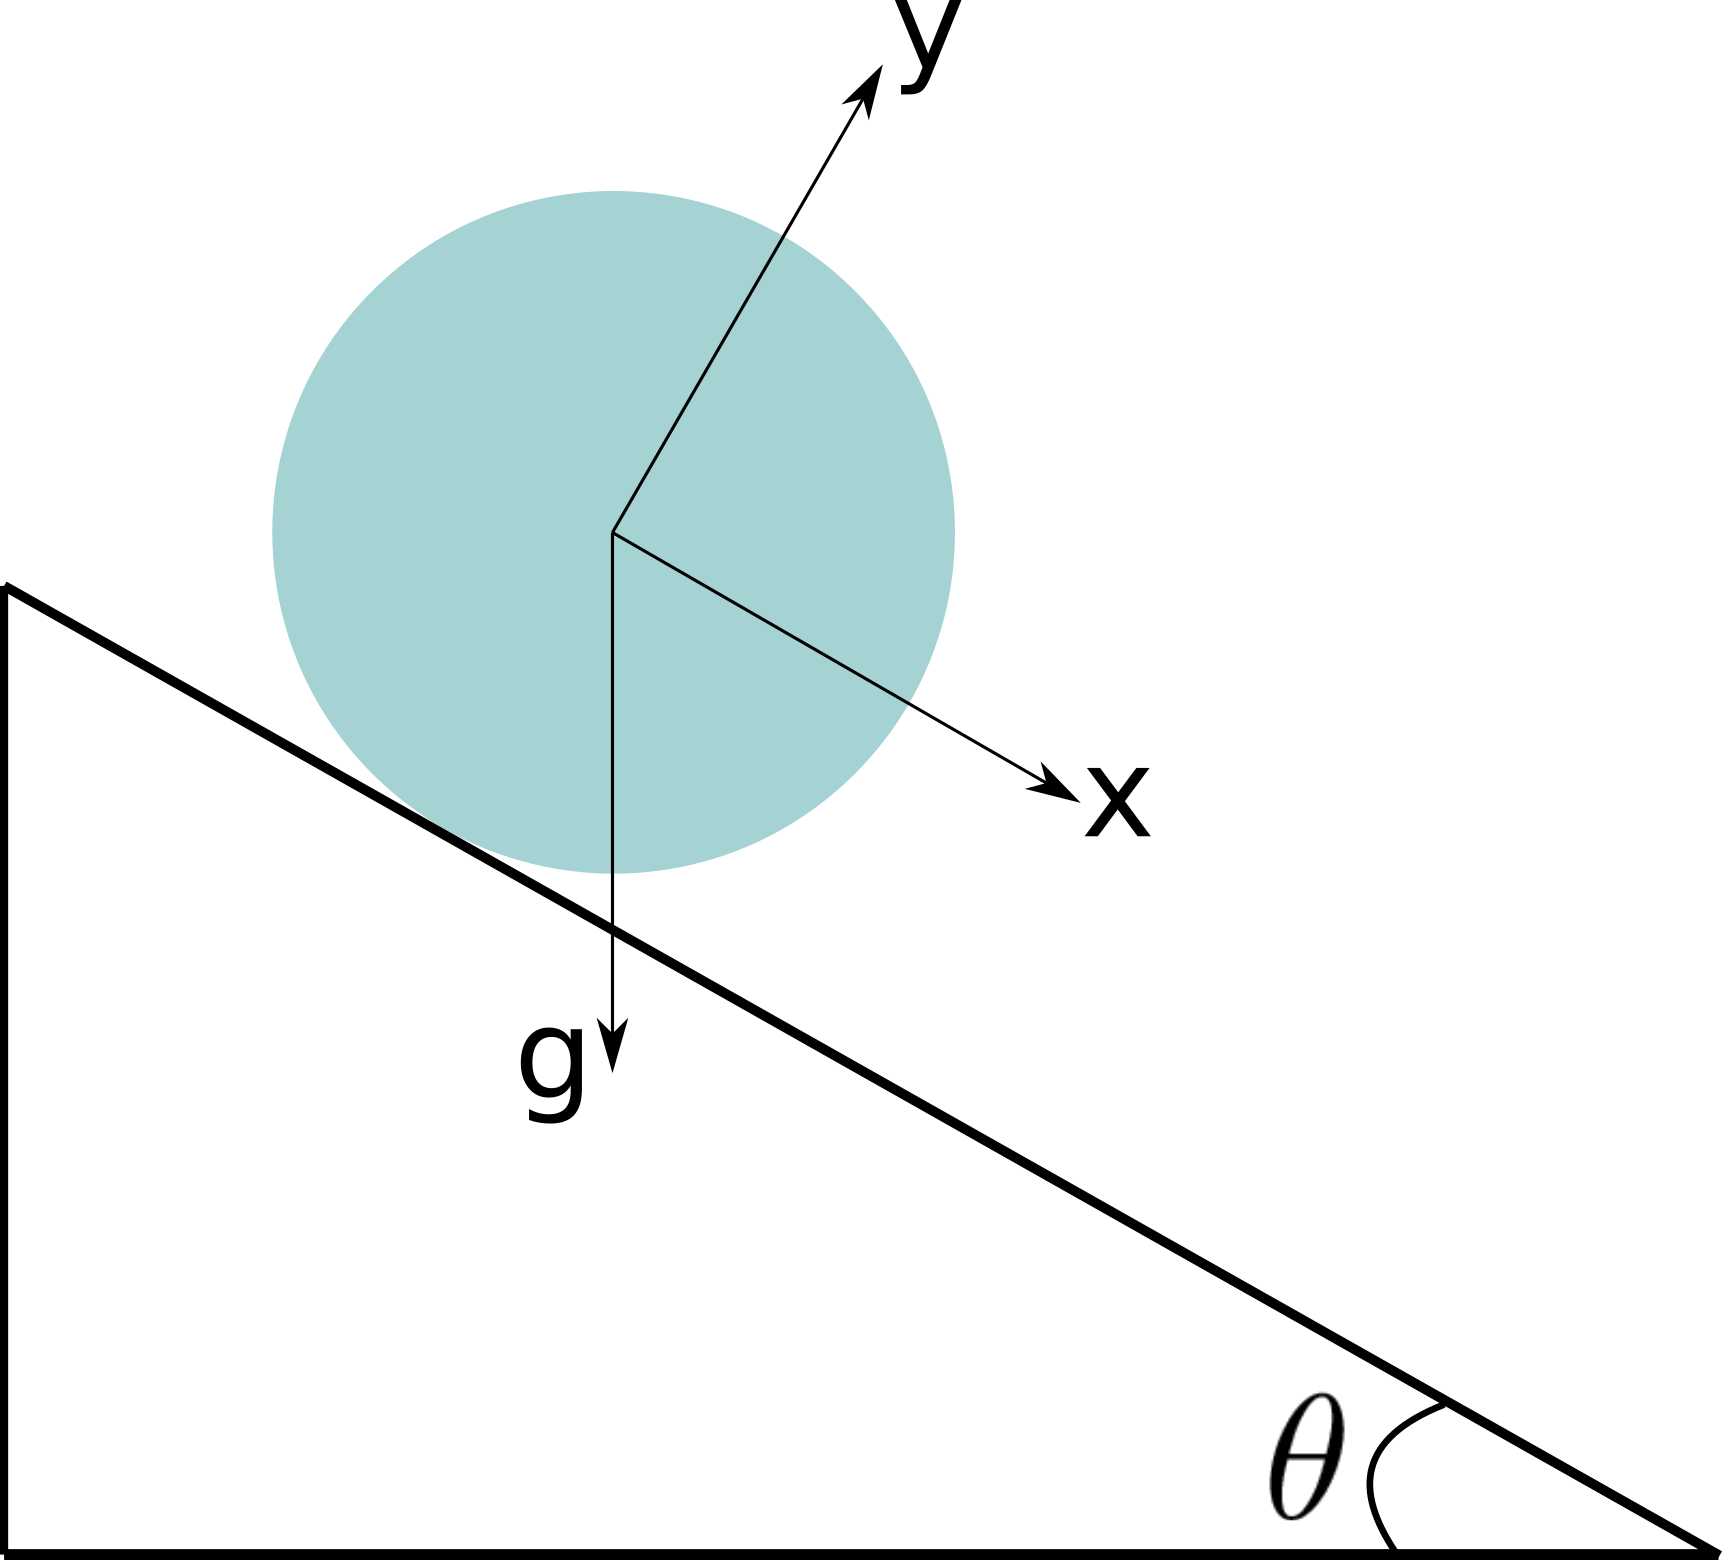
\includegraphics[width=1.0\textwidth]{images/de_2021_cylinder_rolling_on_an_inclined_plane/schematic_1}
    \subcaption{}\label{fig:circular-body:schematic-1}
  \end{subfigure}
  \begin{subfigure}{0.48\textwidth}
    \centering
    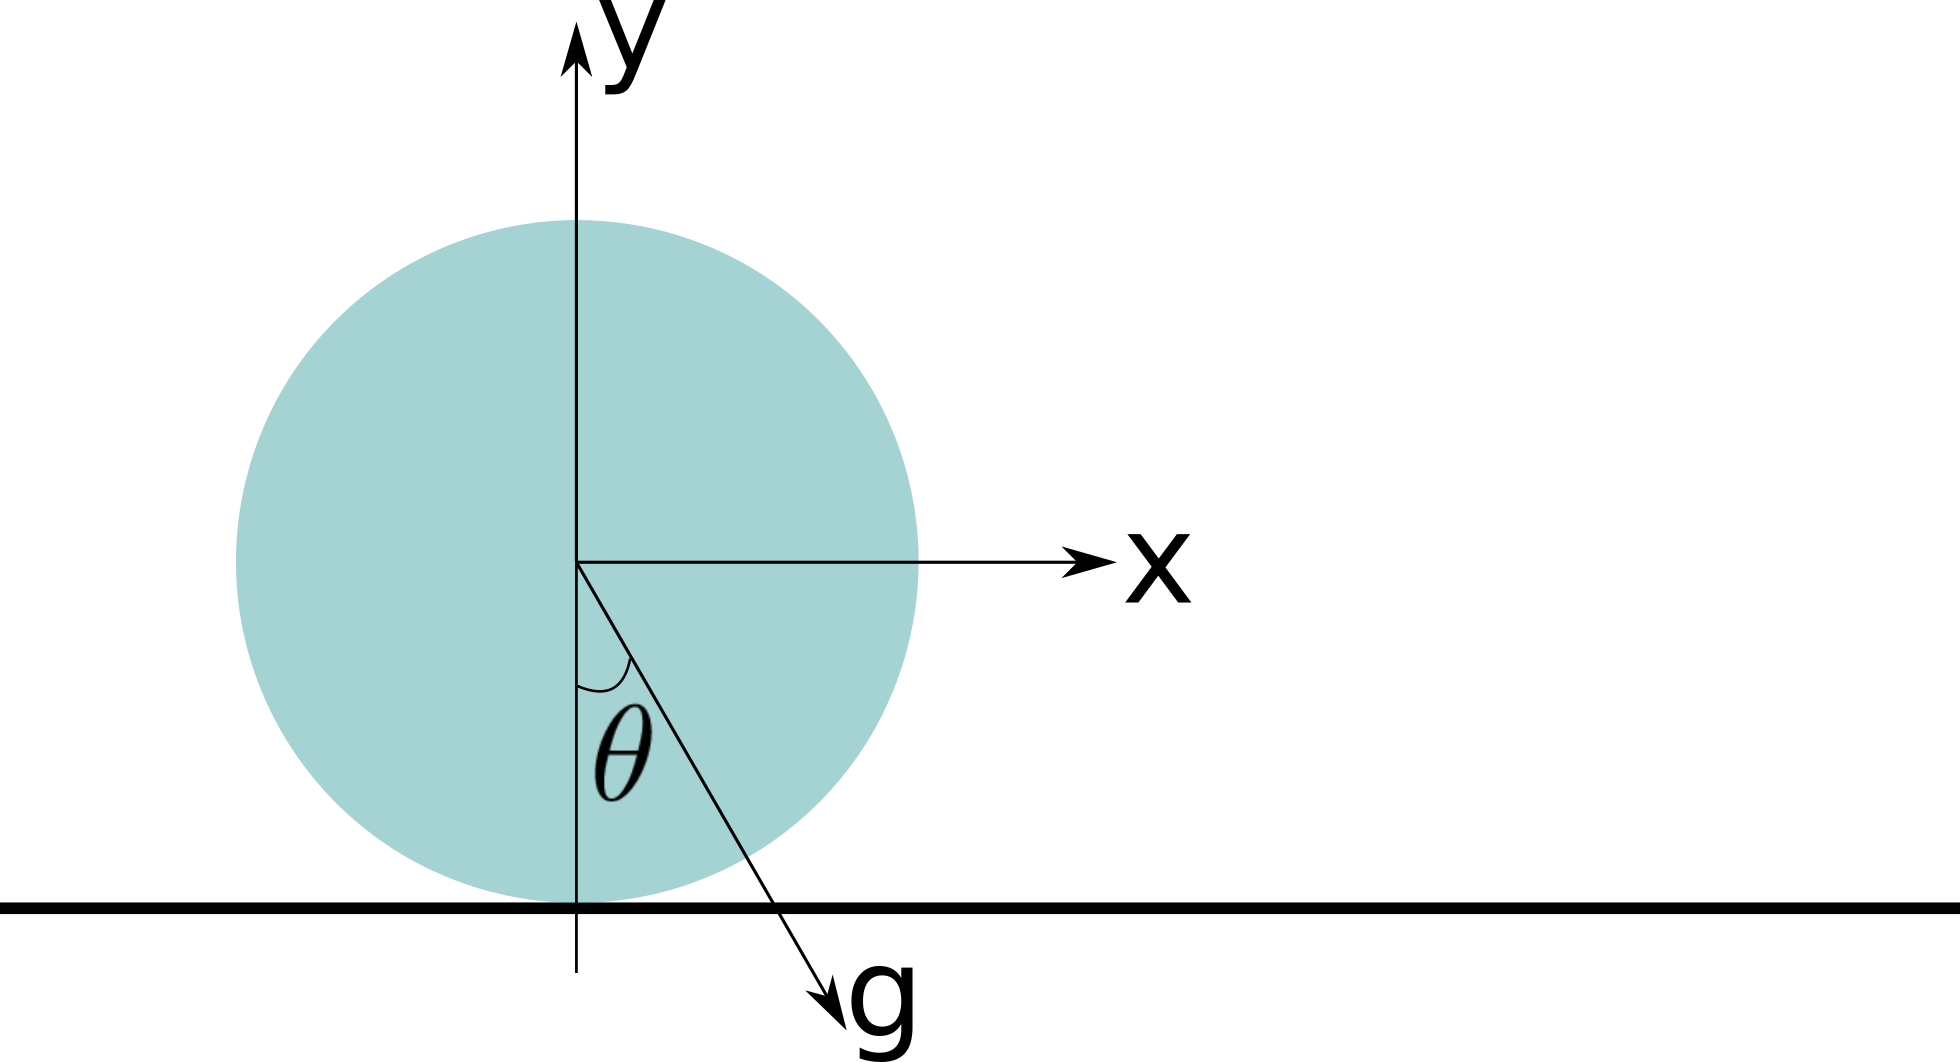
\includegraphics[width=1.0\textwidth]{images/de_2021_cylinder_rolling_on_an_inclined_plane/schematic_2}
    \subcaption{}\label{fig:circular-body:schematic-2}
  \end{subfigure}
  \caption{Curved interface}
\label{fig:circular-body-schematic}
\end{figure}
\begin{table}[!ht]
  \centering
  \begin{tabular}[!ht]{ll}
    \toprule
    Quantity & Values\\
    \midrule
    $\rho$, density & $2700$ kg\,m\textsuperscript{-3} \\
    $\mu$, friction coefficient & $0.3$ \& $0.6$ \\
    Time of simulation & $0.6$ s \\
    Resolution, $\delta x$ & $0.0025$ m\\
    Smoothing length factor, $h/\Delta x$ & 1\\
    gravity $[g_x, g_y, g_z]$ & $[g\,\sin(\theta), g\,\cos(\theta), 0.0]$\\
    $k_r$, Repulsive stiffness coefficient & $1e7$ \\
    $k_f$, Repulsive stiffness coefficient & $1e5$ \\
    $\alpha_{damp}$ & FIXME\\
    \bottomrule
  \end{tabular}
  \caption{Material properties and numerical parameters used for the rolling
    of cylinder on an inclined surface.}%
  \label{tab:circular-body-rolling-params}
\end{table}

\Cref{fig:cylinder-xcom-vs-time-fric-0-3} and
\cref{fig:cylinder-xcom-vs-time-fric-0-3} depicts the variation of center of
mass of the cylinder with time for a friction coefficients of $0.3$ and $0.6$.
From both the figures we can see that the center of mass predicted by the
current solver is at an excellent agreement with the exact solution. Further
\todo{put the right figure} \cref{fig:cylinder-xcom-vs-time-fric-0-3} shows
the snapshots of the cylinder at different time stamps, from which we can see
that the current scheme is stable.

\begin{figure}[!htpb]
  \centering
  \includegraphics[width=0.4\textwidth]{figures/de_2021_cylinder_rolling_on_an_inclined_plane_2d/fric_coeff_0_3/xcom_vs_time}
  \caption{x com vs time of a cylinder with a friction coefficient of $0.3$.}
\label{fig:cylinder-xcom-vs-time-fric-0-3}
\end{figure}

\begin{figure}[!htpb]
  \centering
  \includegraphics[width=0.4\textwidth]{figures/de_2021_cylinder_rolling_on_an_inclined_plane_2d/fric_coeff_0_6/xcom_vs_time}
  \caption{x com vs time of a cylinder with a friction coefficient of $0.6$.}
\label{fig:cylinder-xcom-vs-time-fric-0-6}
\end{figure}


\FloatBarrier%
\subsection{Three bodies colliding}
\label{sec:three-bodies-colliding}


\begin{figure}[!htpb]
  \centering
  % \includegraphics[width=0.4\textwidth]{figures/mohseni_2021_free_sliding_on_a_slope_3d/velocity_vs_time}
  \caption{Schematic of the three rigid body colliding}
\label{fig:schematic-three-rigid-bodies-colliding}
\end{figure}

\begin{figure}[!htpb]
  \centering
  \begin{subfigure}{0.48\textwidth}
    \centering
    \includegraphics[width=1.0\textwidth]{figures/amaro_2019_collision_between_three_rigid_cubes/Mohseni_Vyas/time0}
  \end{subfigure}
  %
  \begin{subfigure}{0.48\textwidth}
    \centering
    \includegraphics[width=1.0\textwidth]{figures/amaro_2019_collision_between_three_rigid_cubes/Mohseni_Vyas/time1}
  \end{subfigure}

  \begin{subfigure}{0.48\textwidth}
    \centering
    \includegraphics[width=1.0\textwidth]{figures/amaro_2019_collision_between_three_rigid_cubes/Mohseni_Vyas/time2}
  \end{subfigure}
  %
  \begin{subfigure}{0.48\textwidth}
    \centering
    \includegraphics[width=1.0\textwidth]{figures/amaro_2019_collision_between_three_rigid_cubes/Mohseni_Vyas/time3}
  \end{subfigure}
\caption{A dummy figure (To be fixed)}
\label{fig:snapshots-three-cubes-colliding}
\end{figure}
%


\FloatBarrier%
\subsection{Stack of cylinders}
\label{sec:stack-of-cylinders}

This test case is used to validate the current solid-solid contact force
model. A stack of cylinders initially at rest are allowed to settle under
gravity in a tank. This is simulated by Zhang (2011), where DEM is used. The
numerical parameters of the current test case are listed in
\Cref{tab:stack-of-cylinders}. The dimensions of the cylinder as well as the
tank are shown in figure (Ref the schematic figure).

\begin{table}[!ht]
  \centering
  \begin{tabular}[!ht]{ll}
    \toprule
    Quantity & Values\\
    \midrule
    $L$, length of the domain & 1 m \\
    Time of simulation & 2.5 s \\
    $c_s$ & 10 m/s \\
    $\rho_0$, reference density & 1 kg/m\textsuperscript{3} \\
    Reynolds number & 200 \& 1000 \\
    Resolution, $L/\Delta x_{\max} : L/\Delta x_{\min}$ & $[100:200]$ \& $[150:300]$\\
    Smoothing length factor, $h/\Delta x$ & 1.0\\
    \bottomrule
  \end{tabular}
  \caption{Parameters used for the Taylor-Green vortex problem.}%
  \label{tab:stack-of-cylinders}
\end{table}

\Cref{fig:snapshots-stack-of-cylinders} presents a set of snapshots
corresponding to the simulation of a stack of cylinders collapsing under
gravity using CTVF-DEM in comparison with the corresponding experimental
photos by Zhang. From the presented figure, the reproduced cylinder's
positions appear to be consistent with those observed in the experiment. From
\Cref{fig:snapshots-stack-of-cylinders}, the current solver has presented
proper level of stability.



\begin{figure}[!htpb]
  \centering
  \begin{subfigure}{0.48\textwidth}
    \centering
    \includegraphics[width=1.0\textwidth]{figures/stack_of_cylinders_2d/Mohseni_Vyas/time0}
  \end{subfigure}
  %
  \begin{subfigure}{0.48\textwidth}
    \centering
    \includegraphics[width=0.75\textwidth]{images/stack_of_cylinders_experimental_images/time0}
  \end{subfigure}

  \begin{subfigure}{0.48\textwidth}
    \centering
    \includegraphics[width=1.0\textwidth]{figures/stack_of_cylinders_2d/Mohseni_Vyas/time1}
  \end{subfigure}
  %
  \begin{subfigure}{0.48\textwidth}
    \centering
    \includegraphics[width=0.75\textwidth]{images/stack_of_cylinders_experimental_images/time1}
  \end{subfigure}

  \begin{subfigure}{0.48\textwidth}
    \centering
    \includegraphics[width=1.0\textwidth]{figures/stack_of_cylinders_2d/Mohseni_Vyas/time2}
  \end{subfigure}
  %
  \begin{subfigure}{0.48\textwidth}
    \centering
    \includegraphics[width=0.75\textwidth]{images/stack_of_cylinders_experimental_images/time2}
  \end{subfigure}

  \begin{subfigure}{0.48\textwidth}
    \centering
    \includegraphics[width=1.0\textwidth]{figures/stack_of_cylinders_2d/Mohseni_Vyas/time3}
  \end{subfigure}
  %
  \begin{subfigure}{0.48\textwidth}
    \centering
    \includegraphics[width=0.75\textwidth]{images/stack_of_cylinders_experimental_images/time3}
  \end{subfigure}
\caption{A dummy figure (To be fixed)}
\label{fig:snapshots-stack-of-cylinders}
\end{figure}
%



\Cref{fig:x-com-stack-of-cylinders,fig:y-com-stack-of-cylinders} presents the
time histories of the x and y components of the center of mass of the
cylinders respectively as well as those from numerical simulations by
SPH-DCDEM as well as MPS-DEM with respect to those from the experiment Zhang.
From the presented figure, the effective center of mass of the cylinders is in
good agreement with the experiment.

\begin{figure}[!htpb]
  \centering
  \includegraphics[width=0.4\textwidth]{figures/stack_of_cylinders_2d/Mohseni_Vyas/xcom}
  \caption{A dummy figure (To be fixed)}
\label{fig:x-com-stack-of-cylinders}
\end{figure}
\begin{figure}[!htpb]
  \centering
  \includegraphics[width=0.4\textwidth]{figures/stack_of_cylinders_2d/Mohseni_Vyas/ycom}
  \caption{A dummy figure (To be fixed)}
\label{fig:y-com-stack-of-cylinders}
\end{figure}


\FloatBarrier%
\subsection{Falling solid in water}
\label{sec:falling-solid-in-water}

In this section, the rigid fluid coupling part of the current solver is
evaluated by simulation of a rigid cube falling in an hydrostatic tank (cite
experimental paper). The CTVF-DEM solver is employed to simulate water entry
of a rigid cube, which is studied experimentally by (cite the paper). The
numerical parameters of the current test case are listed in
\Cref{tab:stack-of-cylinders}. The dimensions of the schematic are shown in
figure.

\begin{table}[!ht]
  \centering
  \begin{tabular}[!ht]{ll}
    \toprule
    Quantity & Values\\
    \midrule
    $L$, length of the domain & 1 m \\
    Time of simulation & 2.5 s \\
    $c_s$ & 10 m/s \\
    $\rho_0$, reference density & 1 kg/m\textsuperscript{3} \\
    Reynolds number & 200 \& 1000 \\
    Resolution, $L/\Delta x_{\max} : L/\Delta x_{\min}$ & $[100:200]$ \& $[150:300]$\\
    Smoothing length factor, $h/\Delta x$ & 1.0\\
    \bottomrule
  \end{tabular}
  \caption{Parameters used for the Taylor-Green vortex problem.}%
  \label{tab:stack-of-cylinders}
\end{table}

A rigid cube of a side length of 30 mm enters the water initially at
hydrostatic state with a velocity of 30 $m/s$ in z-direction.
\Cref{fig:snapshots-falling-solid-in-water} presents a snapshots of the rigid
cube falling in an hydrostatic tank with the current solver as well as
WCSPH-DEM solver as well as the experimental result. From the presented figure
\Cref{fig:snapshots-falling-solid-in-water}, we can see that the pressure
distribution is smooth and the simulation is stable. A zoomed in view near the
rigid cube is presented in \cref{fig:snapshots-falling-solid-in-water-zoomed}
when simulated with WCSPH-DEM and CTVF-DEM. From
\cref{fig:snapshots-falling-solid-in-water-zoomed} we can see that the fluid
particle distribution around the body with CTVF scheme is uniform when
compared with WCSPH, thanks to the implemented transport velocity formulation.

\begin{figure}[!htpb]
  \centering
  \begin{subfigure}{0.48\textwidth}
    \centering
    \includegraphics[width=1.0\textwidth]{figures/qiu_2017_falling_solid_in_water_2d/dx_0_002/time0}
  \end{subfigure}
  %
  \begin{subfigure}{0.48\textwidth}
    \centering
    \includegraphics[width=1.0\textwidth]{figures/qiu_2017_falling_solid_in_water_2d/dx_0_002/time1}
  \end{subfigure}

  \begin{subfigure}{0.48\textwidth}
    \centering
    \includegraphics[width=1.0\textwidth]{figures/qiu_2017_falling_solid_in_water_2d/dx_0_002/time2}
  \end{subfigure}
  %
  \begin{subfigure}{0.48\textwidth}
    \centering
    \includegraphics[width=1.0\textwidth]{figures/qiu_2017_falling_solid_in_water_2d/dx_0_002/time3}
  \end{subfigure}
\caption{A dummy figure (To be fixed)}
\label{fig:snapshots-falling-solid-in-water}
\end{figure}

\begin{figure}[!htpb]
  \centering
  \begin{subfigure}{0.48\textwidth}
    \centering
    \includegraphics[width=1.0\textwidth]{figures/qiu_2017_falling_solid_in_water_2d/dx_0_002/time0}
  \end{subfigure}
  %
  \begin{subfigure}{0.48\textwidth}
    \centering
    \includegraphics[width=1.0\textwidth]{figures/qiu_2017_falling_solid_in_water_2d/dx_0_002/time1}
  \end{subfigure}

  \begin{subfigure}{0.48\textwidth}
    \centering
    \includegraphics[width=1.0\textwidth]{figures/qiu_2017_falling_solid_in_water_2d/dx_0_002/time2}
  \end{subfigure}
  %
  \begin{subfigure}{0.48\textwidth}
    \centering
    \includegraphics[width=1.0\textwidth]{figures/qiu_2017_falling_solid_in_water_2d/dx_0_002/time3}
  \end{subfigure}
  \caption{Zoomed in snapshots of rigid body inside water.}
\label{fig:snapshots-falling-solid-in-water-zoomed}
\end{figure}

\Cref{fig:disp-falling-solid-in-water} presents the time history of the
displacement of the rigid cube with time in comparison with the experimental
result by (cite experimental paper). From the presented figure, the CTVF-DEM
model has reproduced the displacement of the rigid cube with acceptable levels
of stability as well as accuracy.
\begin{figure}[!htpb]
  \centering
  \includegraphics[width=0.4\textwidth]{figures/qiu_2017_falling_solid_in_water_2d/y_cm_vs_time}
  \caption{Center of mass of rigid body vs time compared with experiment}
\label{fig:disp-falling-solid-in-water}
\end{figure}


\FloatBarrier%
\subsection{3D dam breaking flow hitting cubes}

\cite{amaro2019improvement}

In the current case we simulate a 3d dam breaking flow hitting different
configuration of rigid cubes. This is experimentally studied by SPH DCDEM,
where the author used Direct Linear Transform (DLT) to track the cubes as they
move after the impact. A total three rigid body configurations are studied, a
single cube, three cubes and a pyramid configuration, respectively. It is
numerically studied by SPH-DCDEM, MPS-DEM, and (cite some other papers). The
side length of each cube is $3.5$ mm and the material properties are listed in
\cref{tab:material-properties-3d-dam-breaking-flow-hitting-cubes} and the
numerical parameters are given in
\cref{tab:material-properties-3d-dam-breaking-flow-hitting-cubes}. In all the
three cases the fluid is initially allowed to flow by opening a gate which
lifts at a velocity of 3.5 m\,s\textsuperscript{-1}

\begin{table}[!ht]
  \centering
  \begin{tabular}[!ht]{ll}
    \toprule
    Quantity & Values\\
    \midrule
    $L$, length of the domain & 1 m \\
    $\rho_0$, reference density & 1 kg/m\textsuperscript{3} \\
    Reynolds number & 200 \& 1000 \\
    Resolution, $L/\Delta x_{\max} : L/\Delta x_{\min}$ & $[100:200]$ \& $[150:300]$\\
    \bottomrule
  \end{tabular}
  \caption{Parameters used for the Taylor-Green vortex problem.}%
  \label{tab:material-properties-3d-dam-breaking-flow-hitting-cubes}
\end{table}

\begin{table}[!ht]
  \centering
  \begin{tabular}[!ht]{ll}
    \toprule
    Quantity & Values\\
    \midrule
    $L$, length of the domain & 1 m \\
    $\rho_0$, reference density & 1 kg/m\textsuperscript{3} \\
    Reynolds number & 200 \& 1000 \\
    Resolution, $L/\Delta x_{\max} : L/\Delta x_{\min}$ & $[100:200]$ \& $[150:300]$\\
    \bottomrule
  \end{tabular}
  \caption{Parameters used for the Taylor-Green vortex problem.}%
  \label{tab:numerical-properties-3d-dam-breaking-flow-hitting-cubes}
\end{table}

\Cref{fig:snapshots-single-cube-3d-dam-breaking-flow} shows the snapshots of
the rigid cube moving downstream of the tank when interacting with the fluid
flow against the experimental result (cite SPH DCDEM). From
\Cref{fig:snapshots-single-cube-3d-dam-breaking-flow} we can see that the
rigid cube matches well with the experimental result. Further, we compare the
positions of the rigid cube with time in
\Cref{fig:x-position-single-cube-3d-dam-breaking-flow}, against the
experimental results, SPH-DCDEM, MPS-DEM results. It can be seen from figure
\Cref{fig:x-position-single-cube-3d-dam-breaking-flow} that the current solver
is able to provide good accuracy in producing the correct displacement of the
cube and agrees well with the experimental as well as the other numerical
techniques.
\begin{figure}[!htpb]
  \centering
  \includegraphics[width=0.4\textwidth]{figures/mohseni_2021_free_sliding_on_a_slope_3d/velocity_vs_time}
  \caption{Snapshots of a single cube under a 3d dam breaking flow}
\label{fig:snapshots-single-cube-3d-dam-breaking-flow}
\end{figure}
\begin{figure}[!htpb]
  \centering
  \includegraphics[width=0.4\textwidth]{figures/amaro_2019_dam_breaking_flow_hitting_one_cube_3d/case_1/xcom_vs_time}
  \caption{x position of the cube with time for single cube.}
\label{fig:x-position-single-cube-3d-dam-breaking-flow}
\end{figure}

The initial configuration of the dam breaking flow over three cubes is shown
in figure \Cref{fig:snapshots-three-cubes-3d-dam-breaking-flow}.
\Cref{fig:snapshots-three-cubes-3d-dam-breaking-flow} shows the snapshots of
the rigid cubes at different time instants from the start of fluid hit with
the color of the fluid particles representing pressure. From the
\Cref{fig:snapshots-three-cubes-3d-dam-breaking-flow} we can see that the
simulated rigid bodies match well with the experimental observations. We also
compare the x component of the effective center of mass of the three cubes
with time in \Cref{fig:x-position-three-cubes-3d-dam-breaking-flow}, against
the experimental results, SPH-DCDEM, MPS-DEM results. From figure
\Cref{fig:x-position-three-cubes-3d-dam-breaking-flow}, we can see that the
current solve is agrees well with the experimental as well as with the other
numerical method results.
\begin{itemize}
\item Mention at what time does the fluid hits the rigid cubes.
\end{itemize}
\begin{figure}[!htpb]
  \centering
  \includegraphics[width=0.4\textwidth]{figures/mohseni_2021_free_sliding_on_a_slope_3d/velocity_vs_time}
  \caption{Snapshots of a three cubes under a 3d dam breaking flow}
\label{fig:snapshots-three-cubes-3d-dam-breaking-flow}
\end{figure}
\begin{figure}[!htpb]
  \centering
  \includegraphics[width=0.4\textwidth]{figures/amaro_2019_dam_breaking_flow_hitting_three_stacked_cubes_3d/case_1/xcom_vs_time}
  \caption{x position of the cubes with time for three cube.}
\label{fig:x-position-three-cubes-3d-dam-breaking-flow}
\end{figure}
\begin{figure}[!htpb]
  \centering
  \includegraphics[width=0.4\textwidth]{figures/amaro_2019_dam_breaking_flow_hitting_three_stacked_cubes_3d/case_1/ycom_vs_time}
  \caption{y position of the cubes with time for three cube.}
\label{fig:y-position-three-cubes-3d-dam-breaking-flow}
\end{figure}


The placement of the cubes in the pyramid configuration including dimensions,
distance from the left wall and other dimension related information can be
seen in figure \Cref{fig:snapshots-three-cubes-3d-dam-breaking-flow}.
\Cref{fig:snapshots-three-cubes-3d-dam-breaking-flow} shows the snapshots of
the rigid cubes at different time instants and the color coding of the fluid
particles represents pressure. From
\Cref{fig:snapshots-three-cubes-3d-dam-breaking-flow}, it can be seen that the
rigid body positions are in match with the experimental observations. Which is
further validated by doing a quantitative comparison of the x component of
effective center of mass of the six cubes in time against the experimental
results, SPH-DCDEM, MPS-DEM results in
\Cref{fig:x-position-six-cubes-3d-dam-breaking-flow}. From these figures, we
can see that the current solver is in good agreement with the other numerical
and experimental results.
\begin{figure}[!htpb]
  \centering
  \includegraphics[width=0.4\textwidth]{figures/mohseni_2021_free_sliding_on_a_slope_3d/velocity_vs_time}
  \caption{Snapshots of six cubes under a 3d dam breaking flow}
\label{fig:snapshots-six-cubes-3d-dam-breaking-flow}
\end{figure}
\begin{figure}[!htpb]
  \centering
  \includegraphics[width=0.4\textwidth]{figures/amaro_2019_dam_breaking_flow_hitting_six_stacked_cubes_3d/case_1/xcom_vs_time}
  \caption{x position of the cubes with time for six cubes.}
\label{fig:x-position-six-cubes-3d-dam-breaking-flow}
\end{figure}
\begin{figure}[!htpb]
  \centering
  \includegraphics[width=0.4\textwidth]{figures/amaro_2019_dam_breaking_flow_hitting_six_stacked_cubes_3d/case_1/ycom_vs_time}
  \caption{y position of the cubes with time for six cubes.}
\label{fig:y-position-six-cubes-3d-dam-breaking-flow}
\end{figure}


% \subsection{Dam break with body transport}
% \label{sec:dam-break-with-body-transport}

% \citet{wang2019numerical}

% \subsection{Dam break with multiple bodies transport}
% \label{sec:dam-break-with-multiple-bodies-transport}
% \citet{wang2019numerical}


% \subsection{Cylinders in water collapsed under gravity}
% \label{sec:cylinders-collapse-in-water}
% \citet{chen2019coupled}


\section{Conclusions}
\label{sec:conclusions}

\section*{References}
\bibliographystyle{model6-num-names}
\bibliography{references}



\end{document}

%%% Local Variables:
%%% mode: latex
%%% TeX-master: "paper"
%%% fill-column: 78
%%% End:



\begin{enumerate}
\item DOF
\item Variables to describe the state
\item Governing equations
\item Discretization
\item Two coordinate system (Particle positions about these two)
\item Updated state
\item Rotation matrix
\item (a) Describe how the particles are translated to gloabl system from
  local using rotation matrix. Use a figure.
\item (b) Particle positions about new Rr
\item $\omega$ and $\ten{R}$ relation
\item Relation $I$ and $\ten{R}$
\item Integration of governing equations
\item Advantages of representing the body with just boundary particles and
  speed up
\end{enumerate}
